\chapter{Integration}
The primary objective of this work is integrating the hybrid task planner with the surveillance algorithm is to create a robotic system capable of efficiently patrol and manage complex tasks in dynamic environments.This integration aims to leverage the strengths of both systems: the adaptability and responsiveness of the hybrid task planner and the thoroughness and coverage optimization of the surveillance algorithm.

The hybrid task planner brings a structured approach to managing tasks and making decisions based on a hierarchy of objectives. This ensures that the robot can handle both high-priority tasks (like emergency responses) and lower-priority tasks (like routine surveillance) without human intervention.

On the other hand, the surveillance algorithm optimizes the robot's path to maximize coverage of an area. When integrated with the task planner, this ensures that the robot's movements are not just reactive but are also aligned with the overarching goal of efficient area coverage.



\begin{figure}[h]
  \centering
  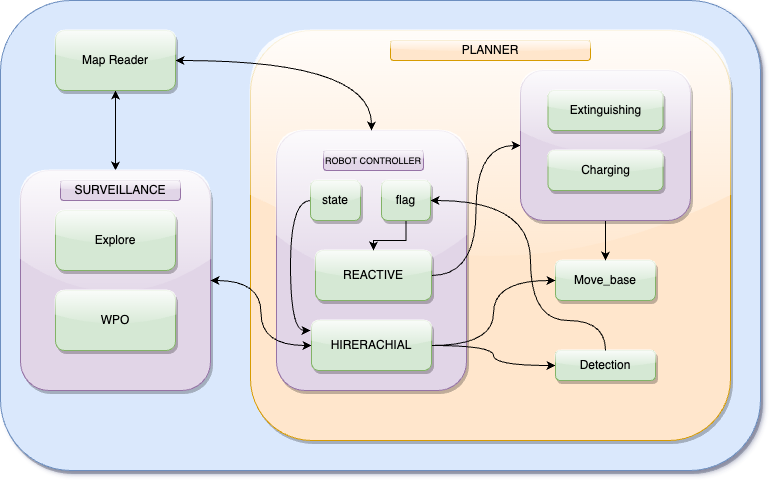
\includegraphics[width=0.9\textwidth, height=0.4\textheight]{Bilder/TPSA.png}
  \caption{TPSA Architecture}
  \label{fig:frontier}
\end{figure}

Integrated Task planner and Surveillance algorithm (TPSA) architecture as shown in \(Figure 7\) has the robot controller component that  encapsulates the task planning and decision-making logic. It monitors the robot's state, battery levels, and external triggers such as fire detection. Based on these inputs, the controller dynamically switches between different operational modes, including direct intervention (like extinguishing fires), recharging, and surveillance.
